% ============================================================================
%  Two-body low-energy scattering — working draft
%  Pedro Henrique Gesualdo Modesto — IFSC/USP
%
%  HOW TO BUILD:      latexmk -pdf main.tex
%  HOW TO CLEAN:      latexmk -c
%
%  YOU NEVER TYPE A NUMBER IN THIS FILE.
%  Every table comes from tables/*.tex and every figure from figures/*.pdf,
%  both written by notebooks/2_dois_corpos/two_body_scattering.ipynb.
%  Re-run the notebook and this document updates itself.
% ============================================================================
% --- Document class -------------------------------------------------------
% article compiles everywhere, so the draft is never blocked. When you submit
% to a Physical Review journal, comment the line below and uncomment the other:
\documentclass[11pt,a4paper]{article}
% \documentclass[twocolumn,amsmath,amssymb,aps,prl]{revtex4-2}

\usepackage[utf8]{inputenc}
\usepackage[T1]{fontenc}
\usepackage{amsmath,amssymb}  % equations
\usepackage{graphicx}         % \includegraphics
\usepackage{booktabs}         % nicer horizontal rules
\usepackage{geometry}         % sane margins
\usepackage{hyperref}         % clickable cross-references
\geometry{margin=2.5cm}
\graphicspath{{figures/}}     % so 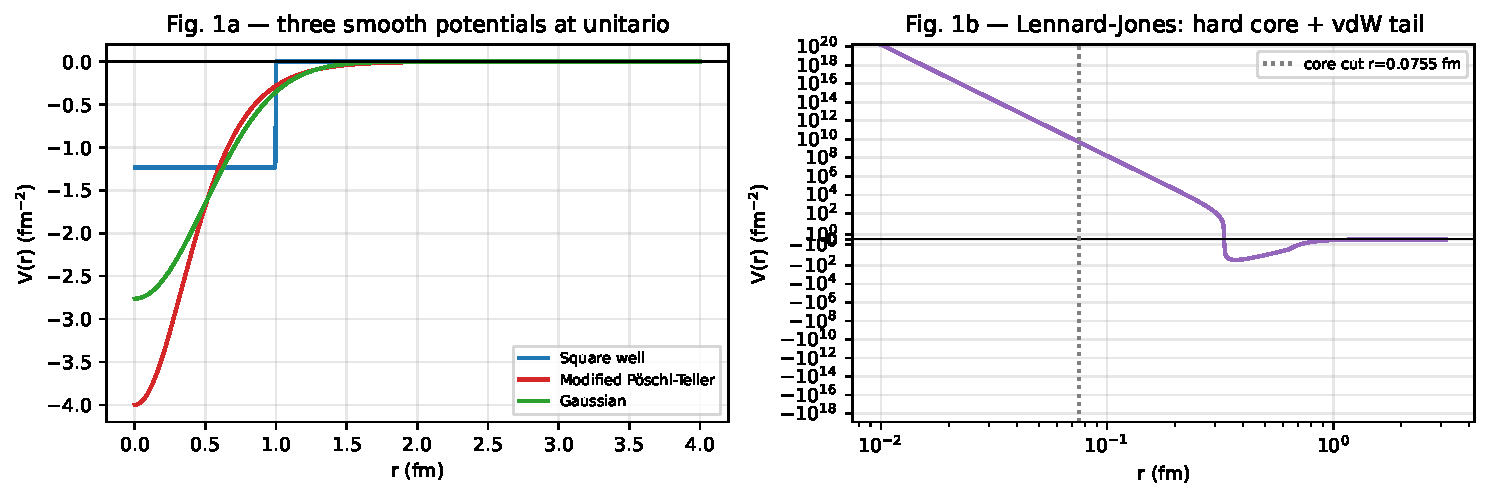
\includegraphics{fig1_potentials} just works

% article has no \affiliation; this fakes it well enough for a draft.
\newcommand{\affiliation}[1]{\\ \small\textit{#1}}

\begin{document}

\title{Shape independence of two-body low-energy observables:\\
       a numerical study across four model potentials}

\author{Pedro Henrique Gesualdo Modesto \and Lucas Madeira
        \affiliation{S\~ao Carlos Institute of Physics, University of S\~ao Paulo}}
\date{\today}

\maketitle

\begin{abstract}
% TODO (write this LAST, after the conclusions).
% Formula that works: context / gap / what we did / the number / what it means.
Placeholder abstract.
\end{abstract}

% ============================================================================
\section{Introduction}
% Placeholder citations so BibTeX has something to do until the text exists.
The reference calculation is Ref.~\cite{macedolima2023}; the physical inputs
come from Refs.~\cite{hackenburg2006,cencek2012}; the three-body continuation
follows Ref.~\cite{madeira2021}.
% TODO. Three paragraphs is enough:
%   1. At low energy only a and r0 survive. Why that matters for cold atoms.
%   2. The open question: how well does it hold, and where does it break?
%   3. What this work does, and the headline number (agreement to ~1%).
% ============================================================================

\section{Method}
\subsection{Radial equation and conventions}
% TODO. hbar = mu_red = 1, u'' = 2(V-E)u, lengths in fm.

\subsection{Extracting $a$ and $r_0$}
% TODO. Straight line outside the range; Simpson for the r0 integral;
% grid aligned to the well edge; Numerov degrades on a discontinuity.

\subsection{The inverse problem}
% TODO. Nested bisection; the root is on 1/a, never on a; node counting.
% Figure 5b is the argument — put it here.

% ============================================================================
\section{Results}

\begin{table}[htbp]
\centering
\small
\caption{Literature values used as targets and benchmarks.}
\label{tab:literature}
\begin{tabular}{lllll}
\hline
quantity & value & unit & source & used for \\
\hline
a (n-p triplet) & 5.411 & fm & Hackenburg, Phys. Rev. C 73, 044002 (2006) & Target of the deuteron tuning. Ref. [23] of RBEF 2023.\\
r0 (n-p triplet) & 1.744 & fm & Hackenburg, Phys. Rev. C 73, 044002 (2006) & Second target of the deuteron tuning.\\
E (deuteron) & -2.224 & MeV & Hackenburg, Phys. Rev. C 73, 044002 (2006) & Experimental benchmark for §4 — not an input.\\
a (4He dimer) & 90.4 & angstrom & Cencek et al., J. Chem. Phys. 136, 224303 (2012) & Target of the helium tuning. Ref. [22] of RBEF 2023.\\
r0 (4He dimer) & 8 & angstrom & Cencek et al., J. Chem. Phys. 136, 224303 (2012) & Second target of the helium tuning.\\
E (4He dimer) & -0.00162 & K & Cencek et al., J. Chem. Phys. 136, 224303 (2012) & Experimental benchmark for §4 — not an input.\\
a (n-n singlet) & -18.5 & fm & Macedo-Lima \& Madeira, Rev. Bras. Ensino Fis. 45, e20230079 (2023), Table 2 & Third tuning case: large NEGATIVE a, no bound state.\\
Published potential parameters & -- & - & Macedo-Lima \& Madeira (2023), Tables 3 and 4 & Initial guesses AND the validation target of §3.\\
v threshold, square well & 1.234 & - & Analytic: pi\textasciicircum{}2/8 = 1.2337 & Exact check of the first bound state in the §5 sweep. \\
\hline
\end{tabular}
\end{table}
   % everything taken from outside, with sources

\begin{figure}[htbp]
  \centering
  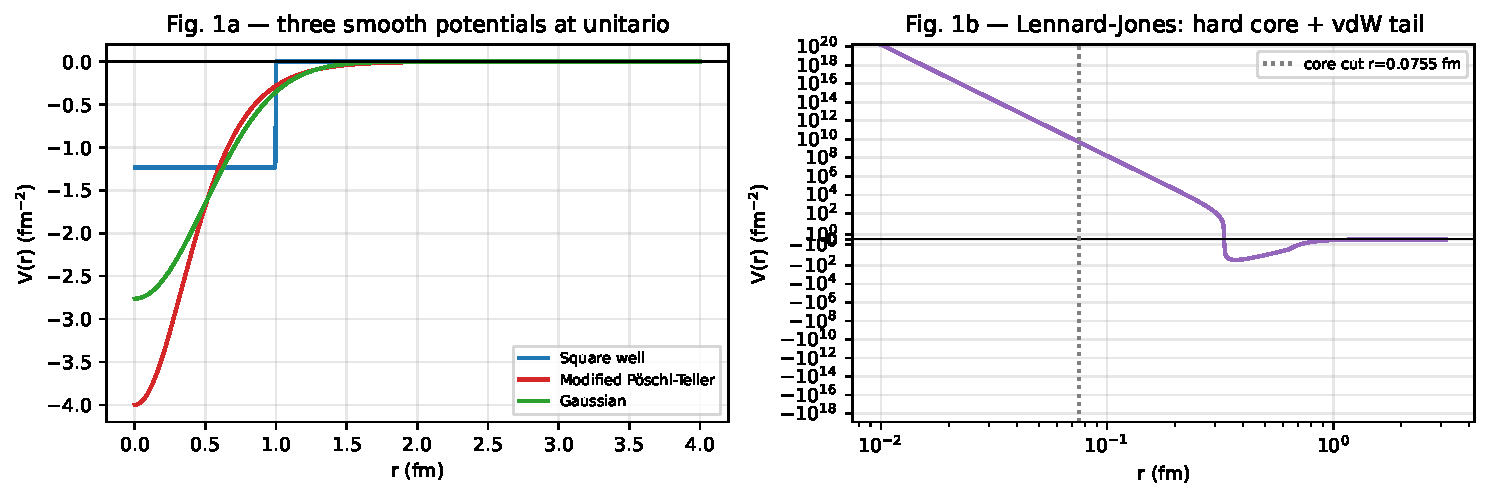
\includegraphics[width=\columnwidth]{fig1_potentials}
  \caption{The four model potentials, all tuned to unitarity.}
  \label{fig:potentials}
\end{figure}

\begin{table}[htbp]
\centering
\small
\caption{Automatic tuning against Tables 3 and 4 of Macedo-Lima and Madeira (2023).}
\label{tab:tuning}
\begin{tabular}{lllllllllll}
\hline
case & potential & p1 & p1 published & p2 & p2 published & a & r0 & nodes & converged & max dev pct \\
\hline
neutron-neutron & Square well & 1.109 & 1.11 & 0.3911 & 0.3918 & -18.5 & 2.7 & 0 & True & 0.1901\\
neutron-neutron & Modified Pöschl-Teller & 0.9071 & 0.9071 & 0.7996 & 0.7991 & -18.5 & 2.7 & 0 & True & 0.06533\\
neutron-neutron & Gaussian & 1.212 & 1.212 & 0.5679 & 0.5672 & -18.5 & 2.7 & 0 & True & 0.1245\\
neutron-neutron & Lennard-Jones & 9.76 & 9.867 & 3.005 & 3.088 & -18.5 & 2.7 & 0 & True & 2.7\\
unitarity & Square well & 1.234 & 1.234 & 0.9998 & 1 & 4.616e+11 & 1 & 0 & True & 0.04152\\
unitarity & Modified Pöschl-Teller & 1 & 1 & 2 & 2 & -2.031e+12 & 1 & 0 & True & 9.497e-09\\
unitarity & Gaussian & 1.342 & 1.342 & 1.435 & 1.435 & -5.912e+12 & 1 & 0 & True & 0.02261\\
unitarity & Lennard-Jones & 0.2646 & 0.2646 & 0.0003407 & 0.0003407 & 3.848e+12 & 1 & 0 & True & 0.003441\\
deuteron & Square well & 1.759 & 1.758 & 0.4992 & 0.5 & 5.4 & 1.7 & 1 & True & 0.1674\\
deuteron & Modified Pöschl-Teller & 1.424 & 1.439 & 0.886 & 0.8631 & 5.4 & 1.7 & 1 & True & 2.653\\
deuteron & Gaussian & 1.911 & 1.91 & 0.6748 & 0.6754 & 5.4 & 1.7 & 1 & True & 0.08625\\
deuteron & Lennard-Jones & 6.84 & 6.815 & 0.9128 & 0.9049 & 5.4 & 1.7 & 1 & True & 0.8746 \\
\hline
\end{tabular}
\end{table}
       % 12 fits vs. the published parameters

\begin{figure}[htbp]
  \centering
  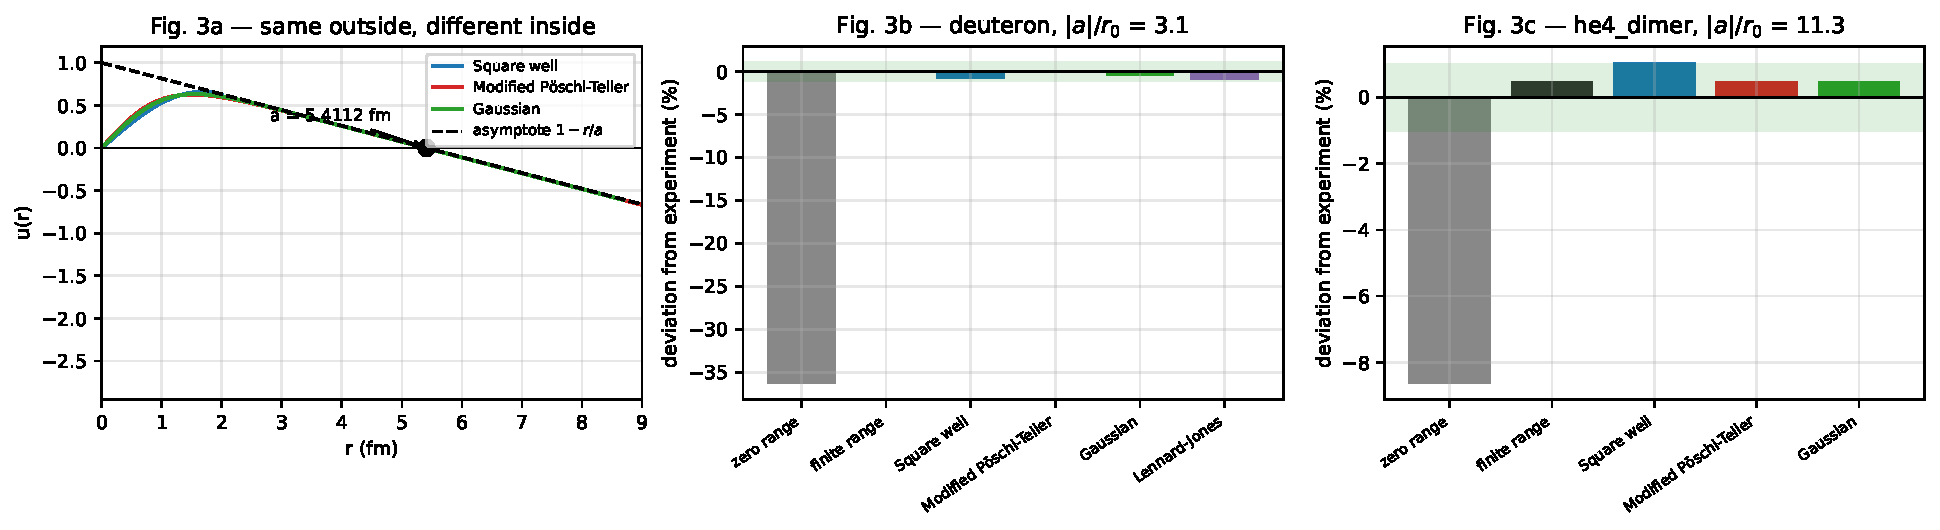
\includegraphics[width=\columnwidth]{fig3_bound_states}
  \caption{Deviation from the measured binding energy. The shaded band is
           $\pm1\%$.}
  \label{fig:bound}
\end{figure}

\begin{table}[htbp]
\centering
\small
\caption{Deuteron binding energy from four tuned potentials.}
\label{tab:deuteron}
\begin{tabular}{llllll}
\hline
method & energy & unit & p1 & p2 & dev pct \\
\hline
experiment & -2.224 & MeV & -- & -- & 0\\
zero range & -1.416 & MeV & -- & -- & -36.33\\
finite range & -2.223 & MeV & -- & -- & -0.05382\\
Square well & -2.206 & MeV & 1.781 & 0.4842 & -0.8191\\
Modified Pöschl-Teller & -2.227 & MeV & 1.444 & 0.8538 & 0.1138\\
Gaussian & -2.214 & MeV & 1.936 & 0.6526 & -0.4691\\
Lennard-Jones & -2.203 & MeV & 7.843 & 1.274 & -0.964 \\
\hline
\end{tabular}
\end{table}

\begin{table}[htbp]
\centering
\small
\caption{Helium dimer binding energy from three tuned potentials.}
\label{tab:helium}
\begin{tabular}{llllll}
\hline
method & energy & unit & p1 & p2 & dev pct \\
\hline
experiment & -0.00162 & K & -- & -- & 0\\
zero range & -0.00148 & K & -- & -- & -8.642\\
finite range & -0.001628 & K & -- & -- & 0.465\\
Square well & -0.001637 & K & 1.333 & 0.1203 & 1.04\\
Modified Pöschl-Teller & -0.001628 & K & 1.075 & 0.2362 & 0.4649\\
Gaussian & -0.001627 & K & 1.446 & 0.171 & 0.4616 \\
\hline
\end{tabular}
\end{table}


\begin{figure}[htbp]
  \centering
  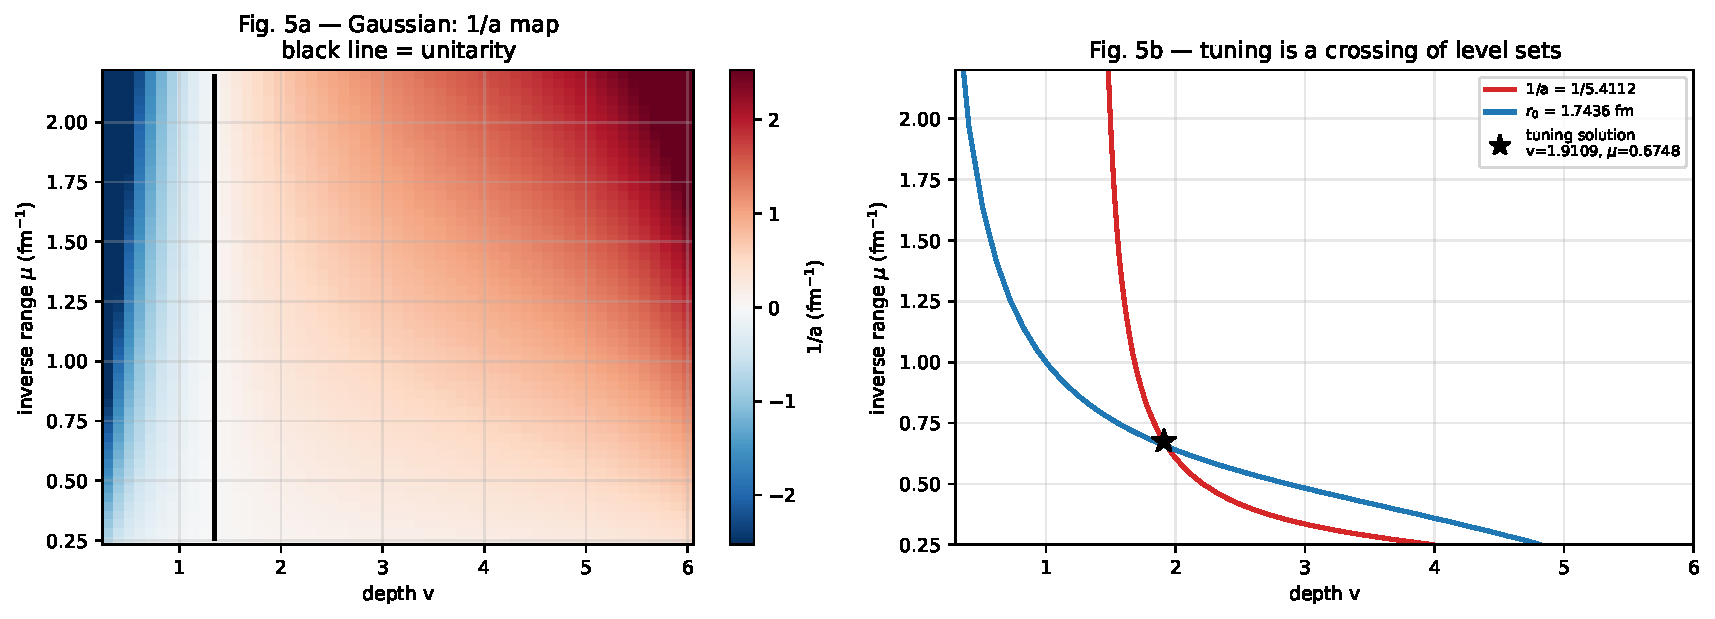
\includegraphics[width=\columnwidth]{fig5_parameter_map}
  \caption{Level sets of $1/a$ and $r_0$; the tuning solution is their crossing.}
  \label{fig:map}
\end{figure}

% ============================================================================
\section{Discussion}
% TODO. The one real finding to defend:
%   |a|/r0 controls everything. Deuteron 3.1 -> zero range misses by 36%.
%   Helium 11.3 -> misses by 8.6%. Adding r0 fixes both to <1%.
%   The residual ~1% spread between potentials IS the shape dependence.

\section{Conclusions}
% TODO.

\section*{Acknowledgments}
This work was supported by CAPES.

% ============================================================================
% Bibliography: run  latexmk -pdf main.tex  and it handles BibTeX for you.
\bibliographystyle{unsrt}
\bibliography{references}
\end{document}
